\section{Analysis}
In this section, we conduct a series of in-depth analyses to better understand the behavior and effectiveness of our \method{} framework. To ensure consistency, all analytical experiments presented here are conducted on the Qwen3-4B-Base model, unless explicitly stated otherwise. Some additional analyses are shown in Appendix~\ref{app:one_model}.


\subsection{Ablation Study}
\label{sec:ablation}
\finding{Removing Repetition Penalty and Task Filtering will harm the final performance.}

\vspace{-10pt}



\begin{wraptable}{r}{0.5\textwidth}
    \vspace{-0.2in} % Adjust vertical spacing if needed
    \centering
    \small
    \caption{Ablation results on Qwen3-4B-Base.  \textbf{w/o Filtering}: Disables the difficulty-based curriculum filtering. \textbf{w/o Rep. Penalty}: Removes the repetition penalty from the Challenger's reward.}
    \label{tab:ablation_study}
    \vspace{-0.1in}
    \begin{tabular}{@{}lcc@{}}
        \toprule
        \textbf{Method} & \textbf{Math AVG} & \textbf{General AVG} \\
        \midrule
        \method{} & 49.07 & 31.15 \\
        \midrule
        \textit{Ablations} & & \\
        % \quad $\vdash$ w/o RL-Challenger & 44.36 & 26.32 \\
        \quad $\vdash$ w/o Rep. Penalty  & 45.76 & 28.73 \\
        \quad $\vdash$ w/o Filtering     &   47.35  &   26.69  \\
        \bottomrule
    \end{tabular}
    \vspace{-0.15in}
\end{wraptable}

To isolate the contribution of each key component within our \method{} framework, we conduct a comprehensive ablation study on the \texttt{Qwen3-4B-Base} model. We specifically investigate the importance of two critical modules by disabling them one at a time and observing the impact on performance. The results are summarized in Table~\ref{tab:ablation_study}.

As shown in the table, removing any core components leads to a significant degradation in performance. 
Removing the \textbf{Repetition Penalty} harms performance, indicating that generating a diverse set of questions is crucial for effective Solver training. 

Finally, disabling the \textbf{Task Filtering} module results in a notable performance drop, particularly on the general-domain average, which falls by over 6 points. As discussed in Section~\ref{sec:data_gen}, this filtering serves a dual purpose: it calibrates the curriculum's difficulty and acts as an implicit quality control mechanism by removing questions with low answer consistency. Without this filter, the Solver is trained on noisy data that likely includes ambiguous or ill-posed questions, which harms its ability to learn robustly.



% Finally, despite this drop in absolute label accuracy, the framework's internal reward mechanism functions precisely as designed. The scores on the table's diagonal show how each Solver performs on questions from its contemporary Challenger. The Solver (Step 30) achieves 51.5\% and the Solver (Step 45) achieves 50.5\% on their respective question sets. This demonstrates that the Challenger successfully calibrates the question difficulty to match the Solver's evolving capabilities, consistently targeting the 50\% success rate that our reward function incentivizes.

% \subsection{Limitations and Performance Degradation}
% \label{sec:analysis_degradation}

% While our framework demonstrates strong initial gains, our extended experiments reveal a clear performance trajectory that defines its practical limits. We tracked the average performance on both math and general-domain benchmarks, alongside the true accuracy of the self-generated pseudo-labels, for five full iterations. 

% \begin{table}[ht]
%     \centering
%     \small
%     \caption{Performance metrics tracked over five training iterations. The table lists the true accuracy of the pseudo-labels for each iteration, alongside the resulting model's average performance on math and general-domain benchmarks.}
%     \label{tab:performance_degradation}
%     \begin{tabular}{@{}lccc@{}}
%         \toprule
%         \textbf{Iteration} & \textbf{Pseudo-Label Acc.} & \textbf{Math Average} & \textbf{General Average} \\
%         \midrule
%         1 & 79.0\% & 48.06 & 29.68 \\
%         2 & 69.0\% & 48.44 & \textbf{30.41} \\
%         3 & 63.0\% & \textbf{49.07} & 29.83 \\
%         4 & 54.0\% & 46.52 & 29.30 \\
%         5 & 47.0\% & 45.58 & 29.28 \\
%         \bottomrule
%     \end{tabular}
% \end{table}

% Table~\ref{tab:performance_degradation} reveals that the model's capabilities on math problems peak at the third iteration and subsequently begin to \textit{degrade}. This degradation is particularly pronounced on the math benchmarks, which are the direct target of our self-generated curriculum. In contrast, the performance on general-domain tasks remains relatively stable, showing only a minor decline.

% We attribute this performance drop directly to the decline in the quality of the self-generated pseudo-labels. As shown in the table, the pseudo-label accuracy falls from a high of 79.0\% to just 47.0\% by the fifth iteration. After a certain point, the level of noise from these inaccurate labels becomes harmful. The Solver begins to learn from a random training signal, which not only halts progress but actively damages its previously acquired mathematical reasoning skills. This self-poisoning dynamic illustrates the inherent risk of a fully autonomous self-improvement loop when data fidelity is not explicitly managed.

% This finding suggests a potential path for future improvement. The performance degradation is not a fundamental flaw of the co-evolutionary concept itself, but rather a consequence of the base model's initial capabilities. \textit{Starting with a more powerful base model would likely mitigate this issue}. A stronger initial model would generate more accurate pseudo-labels from the outset, thus maintaining a higher-quality training signal for more iterations and significantly extending the effective training runway before performance begins to degrade.

\subsection{Iteration Scaling}
\finding{Model performance eventually converges, with the timing depending on model size.}
% \vspace{-10pt}
Previous results demonstrate that ~\method{} enhances the Solver's capabilities. This raises a critical question about the long-term stability of our self-improvement loop: \textit{what are the limits of this process, and whether the eventual performance degradate?} In this section, we conduct an analysis to investigate these iteration scaling dynamics, aiming to diagnose the underlying cause of this instability.


% \subsubsection{The Inevitability of Collapse: An Empirical Analysis}


\begin{wrapfigure}{r}{0.5\textwidth} 
    \vspace{-0.2in}
    \centering
    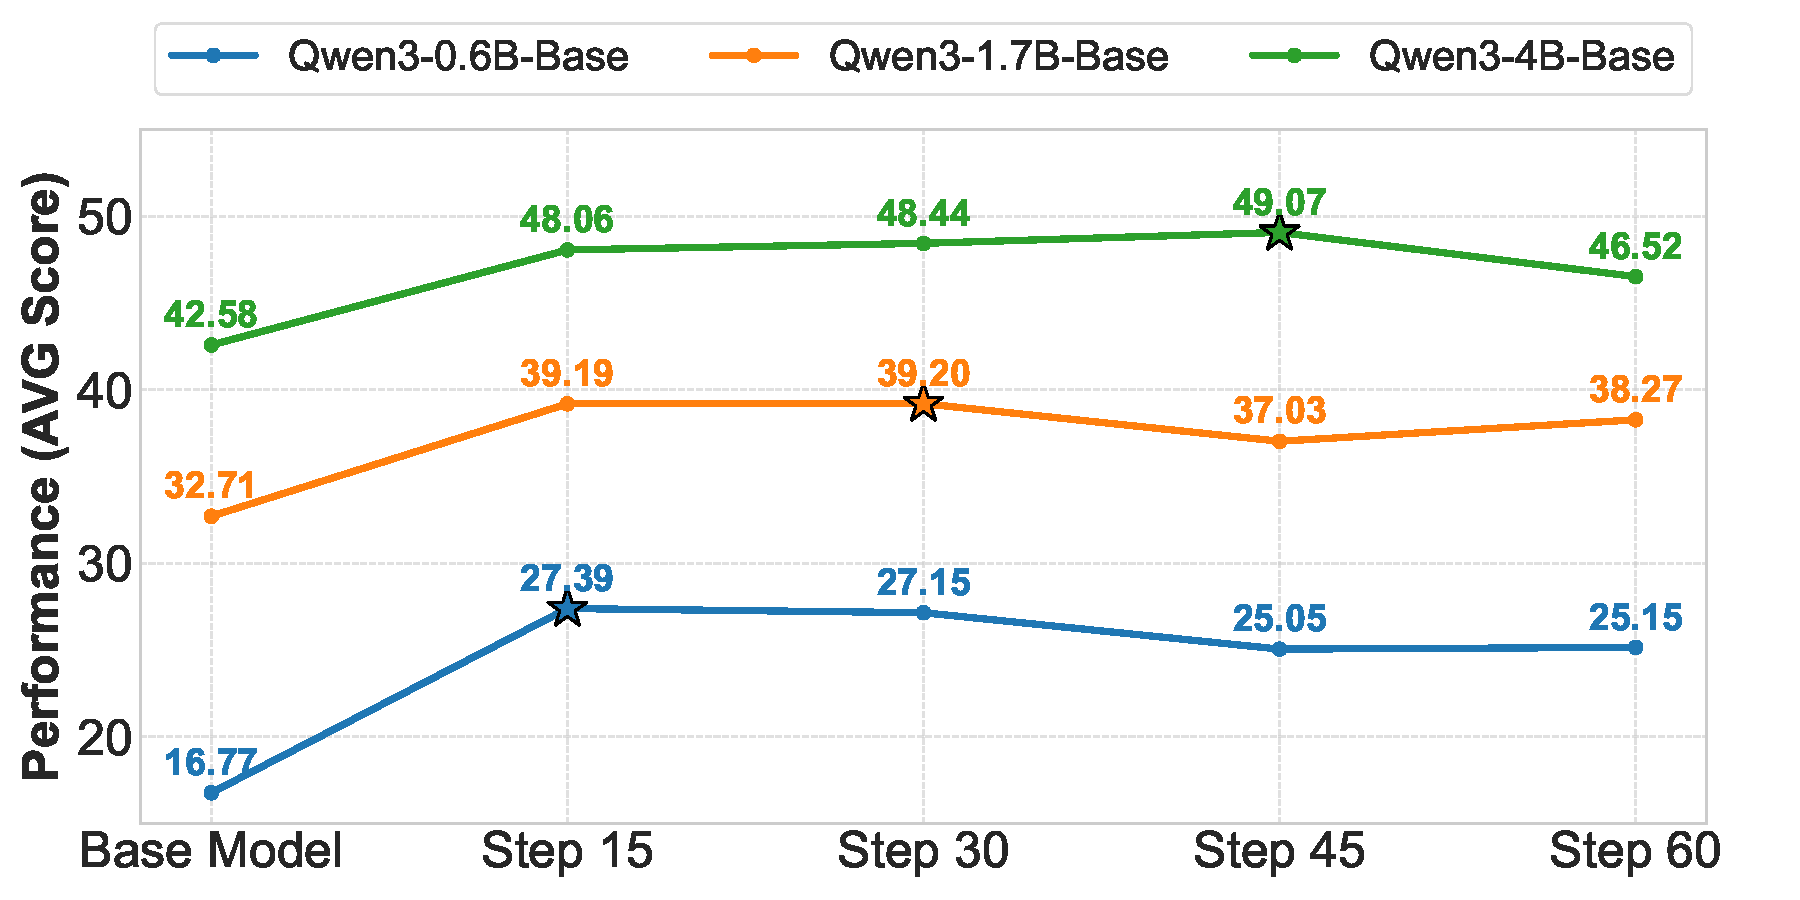
\includegraphics[width=\linewidth]{figures/scaling.pdf}
    \vspace{-0.25in}
    \caption{Math performance across different iteration times and model scales. The star markers indicate the peak performance for each model size.}
    \label{fig:performance_collapse_chart}
    \vspace{-0.2in} % Reduce space below the figure and caption
\end{wrapfigure}


As illustrated in Figure \ref{fig:performance_collapse_chart}, our framework initially delivers on its promise, with models of all sizes showing significant performance improvements in the early stages of co-evolution. Unfortunately, this virtuous cycle does not continue indefinitely. After multiple iterations, we observe a consistent and concerning trend of performance degradation across all models. Intriguingly, we found a direct correlation between model scale and resilience to this collapse: the larger the model, the later the onset of performance degradation.

For instance, the smallest 0.6B model reaches its peak performance as early as the first iteration (Step 15), after which its capabilities begin to decline. In contrast, the largest 4B model sustains its upward trajectory for three full iterations, only experiencing a sharp drop at Step 60. This pattern strongly suggests that while larger model capacity can delay the negative effects, it does not prevent them. This eventual collapse points to an inherent instability or limitation within our current self-improvement framework, highlighting a critical area for future investigation. We present some additional analysis results for this in Appendix~\ref{app:scaling_ana}.



\subsection{Synergy with Supervised Data}
\label{sec:analysis_synergy}
\finding{Using R-zero as a mid-training method boosts the effect of later training on human data.}
\vspace{-10pt}
To analyze the utility of our framework in scenarios where a labeled dataset is available, we measure the synergy between \method{} and traditional supervised fine-tuning using labeled datasets~\footnote{\url{https://huggingface.co/datasets/hiyouga/math12k}}. The GRPO settings for this experiment were kept identical to our main experiments.

% \begin{wrapfigure}{r}{0.45\textwidth}
%     \vspace{-10pt} % Add a negative vertical space to pull the figure up slightly
%     \centering
%     \includegraphics[width=\linewidth]{figures/humanlabel.pdf}
%     % \vspace{-0.3in}
%     \caption{Performance of \method{} when combined with supervised fine-tuning. The dashed line represents the baseline of fine-tuning the base model on labelled data alone, showing that our iterative method provides a better initialization.}
%     \label{fig:synergy_with_sft}
%     % \vspace{-15pt} % Add a negative vertical space to reduce space below the figure
%     \vspace{-0.3in}
% \end{wrapfigure}

\begin{figure}[h]
    \centering
    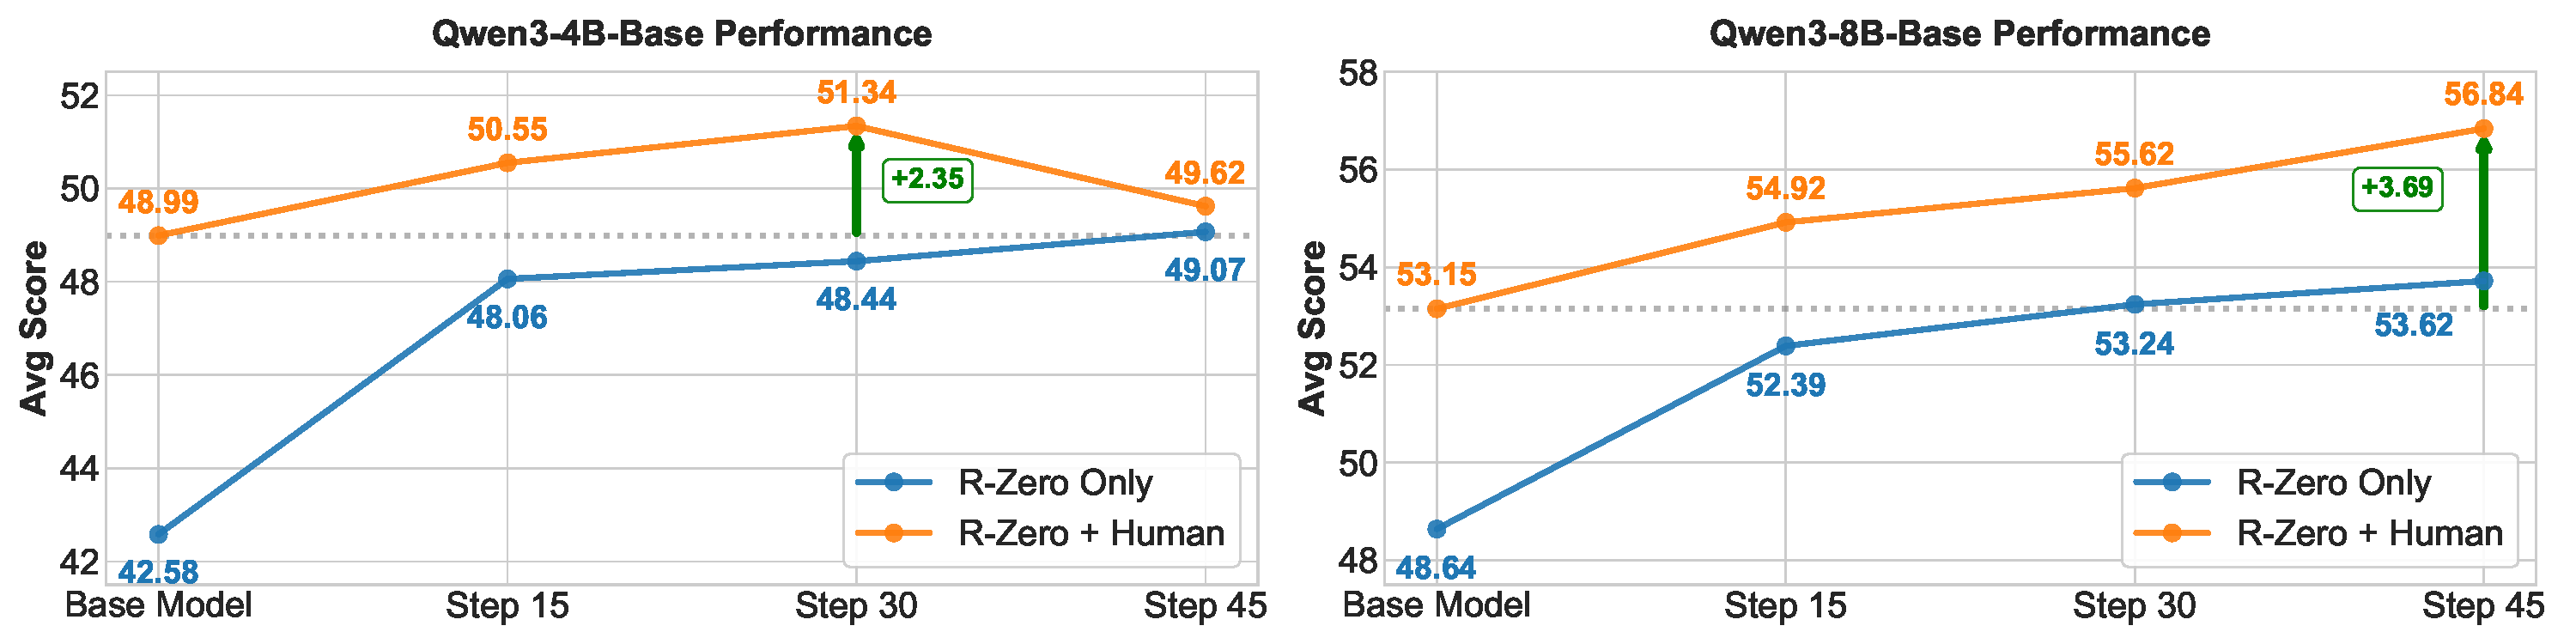
\includegraphics[width=0.95\linewidth]{figures/comparison_split_adjusted_v3.pdf}
    \caption{Performance of \method{} when combined with supervised fine-tuning. The dashed line represents the baseline of fine-tuning the base model on labelled data alone, showing that our iterative method provides a better initialization.}
    \label{fig:synergy_with_sft}
    % \vspace{-0.3in}
\end{figure}

We first establish a supervised baseline by fine-tuning the base model directly on the labeled data. For this process, we also employ GRPO.

% \todo[inline]{HM: Here supervised baseline is Zero-RL? The original data are prompt-answer pairs, which are only for RL. And the base model is~\texttt{Qwen3-4B-Base}?}
We then apply our \method{} framework, where at the end of each co-evolutionary iteration, the resulting checkpoint is also fine-tuned on the same labeled dataset. The results show that our method provides significant additional gains. As highlighted in  Figure~\ref{fig:synergy_with_sft}, this represents a gain of \textbf{+2.35 points} over the human-label-only baseline for 4B model.

This finding confirms that \method{} is not redundant with labeled data; instead, it acts as a powerful performance amplifier. The co-evolutionary process enables the model to better leverage the supervised information and achieve performance levels unattainable by standard fine-tuning alone.

\textcolor{black}{
We also studied the scenario where human-labeled datasets are mixed into the R-Zero generated dataset for training. 
We found that this concurrent training approach outperforms using either R-Zero dataset or humanlabel dataset alone, 
but it does not surpass the sequential strategy of first applying R-Zero and then performing SFT. 
We hypothesize that mixing the labeled data during R-Zero training may dilute the high-quality signal while partially mitigating noise. 
Performing R-Zero first allows the model to acquire reasoning ability before leveraging the high-quality human-labeled data, 
which appears to be the most effective strategy. 
The precise underlying reasons require further investigation.}
\begin{table}[h!]
\tiny
\centering
\rowcolors{1}{white}{white}
{\color{black}
\begin{tabular}{lcccccccccc}
\toprule
Dataset & AMC & Minerva & MATH & GSM8K & Olympiad & AIME25 & AIME24 & SuperGPQA & MMLU-Pro & BBEH \\
\midrule
Human          & 57.97 & 55.15 & 80.8  & 92.04 & 48    & 9.58  & 10.31 & 29.49 & 57.03 & 9.71  \\
\method{}      & 57.27 & 52.94 & 79.6  & 92.12 & 44.59 & 9.6   & 13.4  & 27.55 & 55.47 & 10.42 \\
\method{}+Human & 57.9  & 53.2  & 81.2  & 92.2  & 47.7  & 10.32 & 14.67 & 29.4  & 58.2  & 11.8  \\
\bottomrule
\end{tabular}
}

\caption{\textcolor{black}{Performance comparison across benchmarks when training with human-labeled data, R-zero self-generated data, and a mixed training strategy.}}
\end{table}










\subsection{Evolution of Question Difficulty and Data Accuracy}
\label{sec:analysis_difficulty_accuracy}
\finding{Question difficulty increases progressively with decreasing pseudo-label accuracy.}
\vspace{-10pt}
\begin{table}[h!]
    \centering
    \small
    \caption{Performance and data accuracy analysis. The highlighted column represents the \textit{true accuracy} of the self-generated pseudo-labels for each question set.}
    \label{tab:difficulty_evolution}
    % \vspace{-0.1in}
    \begin{tabular}{@{}lcccc>{\columncolor{gray!15}}c@{}}
        \toprule
        & \multicolumn{5}{c}{\textbf{Performance of Evaluated Model (vs. Ground Truth)}} \\
        \cmidrule(l){2-6}
        & Base Model & Solver (step 15) & Solver (step 30) & Solver (step 45) & Pseudo-Label Acc. \\
        \midrule
        $\mathcal{D}_{\text{Step 15}}$ & 48.0 & 59.0 & 57.0 & 61.0 & 79.0\% \\
        $\mathcal{D}_{\text{Step 30}}$ & 52.5 & 53.0 & 51.5 & 53.5 & 69.0\% \\
        $\mathcal{D}_{\text{Step 45}}$ & 44.0 & 47.0 & 45.0 & 50.5 & 63.0\% \\
        \bottomrule
    \end{tabular}
\end{table}



To understand the co-evolutionary dynamic, we analyzed how the Challenger's generated questions and their corresponding pseudo-labels change across iterations. We sampled 200 questions from the Challenger's policy after each of the first three training iterations, creating three distinct test sets: $\mathcal{D}_{\text{step 15}}$, $\mathcal{D}_{\text{step 30}}$, and $\mathcal{D}_{\text{step 45}}$. For this analysis, we assumed the external oracle model, GPT-4o, to be a perfect annotator, providing the ground truth answers for all generated questions.

The evaluation was conducted as follows: the performance of our internal models was measured against these GPT-4o ground truth answers. The score reported for GPT-4o itself, however, reflects the \textbf{true accuracy of our self-generated pseudo-labels} by comparing the pseudo label against the ground truth from the oracle (GPT-4o). The results on the filtered dataset are summarized in Table~\ref{tab:difficulty_evolution}.


% \todo[inline]{HM: In Table~\ref{tab:difficulty_evolution}, shall we use  $\mathcal{D}_{\text{Iter x}}$ instead of Challenger (Iter x). }

This analysis reveals a multi-faceted dynamic. The first finding is that the questions generated by the Challenger become \textbf{progressively more difficult}. This is directly evidenced by evaluating a fixed model against the evolving question sets. For instance, the performance of the static Solver (Step 15), when measured against the consistent GPT-4o ground truth, drops from 59.0\% on the questions for the Step 15 training to 47.0\% on the questions for the Step 45. This confirms that the Challenger is successfully increasing the intrinsic difficulty of its curriculum.

The second finding, revealed by the highlighted column, pertains to the \textbf{true accuracy of the self-generated dataset}. Unfortunately, while the accuracy of the pseudo-labels is initially high at 79.0\%, it systematically drops to 63.0\% by the third iteration. This trend indicates that as the system generates more difficult problems, the Solver's majority vote becomes a less reliable source for ground truth. This decline in data quality is a critical trade-off and a potential bottleneck for the framework's ultimate performance.
